\documentclass[useAMS,usenatbib]{mn2e}
\usepackage{graphicx}
\usepackage{amssymb}
\usepackage{natbib}
\bibliographystyle{mn2e}
\pdfminorversion=5   % recommended by MNRAS web page


%%% Journal abbreviations.
\def\apj{ApJ}                 % Astrophysical Journal
\def\apjl{ApJL}               % Astrophysical Journal, Letters
\def\apjs{ApJS}               % Astrophysical Journal, Supplement
\def\mnras{MNRAS}             % Monthly Notices of the RAS
\def\aap{A\&A}                % Astronomy and Astrophysics
\def\aaps{A\&AS}              % Astronomy and Astrophysics, Supplement
\def\aj{AJ}                   % Astronomical Journal
\def\physrep{Phys.~Rep.}      % Physics Reports
\def\nat{Nature}              % Nature
\def\araa{ARA\&A}             % Annual Review of Astronomy and Astrophysics
\def\planss{planss}           % Planetary and Space Science
\def\ssr{SSR}                 % Space Science Reviews
\def\sovast{Sov.~Astron.}     % Soviet Astronomy
\def\canjphys{Can. J. Phys.}  % Canadian Journal of physics
\def\nar{New~Astron.}

 
\newcommand{\msun}{{M$_\odot$}}

\topmargin -1cm


\title{Cooling Clouds by Varying Metallicities: Origin of Globular Cluster Bimodality}

\author[R. Fernandez et al.]{Ricardo Fernandez$^{1}$ and Greg L. Bryan$^{1}$\\
$^{1}$Department of Astronomy, Columbia University, 550 West 120th Street, New York, NY 10027, USA}

\begin{document}

\date{}

%\pagerange{\pageref{firstpage}--\pageref{lastpage}} \pubyear{2013}

\maketitle

%\label{firstpage}

\begin{abstract}
Globular Clusters
\end{abstract}

\begin{keywords}
globular clusters - methods:numerical
\end{keywords}

%% ----------------------------------------------------------------
%
\section{Introduction}

%% ----------------------------------------------------------------
%
\section{Basic Idea}
\label{sec:basic}

%% ----------------------------------------------------------------
%
\section{Numerical Models}
\label{sec:numerical}
\subsection{Numerical Method}
This simulations were performed with the publicly available Eulerian three-dimensional
hydrodynamical adaptive mesh refinement Enzo code \citep{Bryan2013}. The domain
box size of the simulation was 150 pc with a top level root grid resolution of $128^3$.
Cell refinement was dictated by baryon mass and Jeans length with a maximum refinement
level of 3. Our simulations included self gravity and radiative cooling using the
Grackle library; details described in \cite{Bryan2013}. The metal heating and
cooling rates are provided from \cite{Haardt2012}.

\subsection{Initial Conditions}
Our initial conditions consisted of a cloud in pressure equilibrium with an
ambient density and temperature background. The internal structure of the
cloud is modeled by a Bonner-Ebert sphere \cite{Bonnor1956}; a self-gravitating
isothermal gas sphere in hydrostatic equilibrium embedded in a pressurized  
medium. To fully describe a Bonner-Ebert sphere, a mass $M_{BE}$, temperature
$T_{BE}$, and an external pressure $P_{ext}$ must be chosen. Following our
assumptions outlined in Section~\ref{sec:basic}, we choosed
$M_{BE}=10^6$ \msun, $T_{BE}=6000$ K, and $P_{ext}=1.8\times10^5\times k_B$
($k_B$ : Boltzmann constant). This corresponds to a cloud on the cusp where
heating and cooling balance. 

In addition, we add turbulence to the cloud following a power spectrum of
$v_k^2 \propto k^{-4}$ for the velocity field.

%% ----------------------------------------------------------------
% 
\section{Results}
\label{sec:results}
\subsection{No Heating Runs}
\begin{figure}
\begin{center}
\includegraphics[width=8.5cm]{Images/density_series}
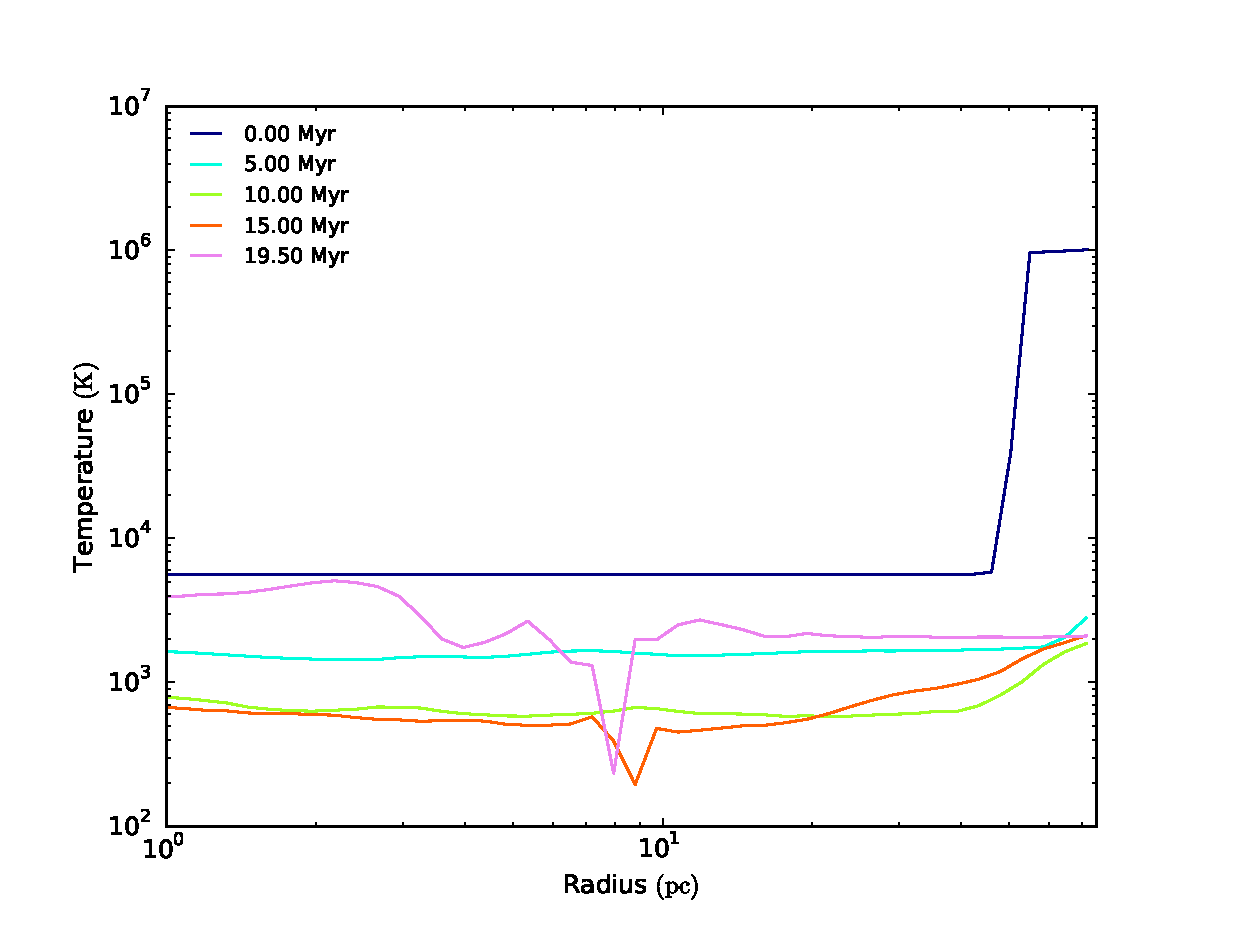
\includegraphics[width=8.5cm]{Images/temperature_series}
\end{center}
\caption{\label{fig:profile_turbulence}} Cell weighted profiles for density
and temperature at give output times for run with cooling, turbulence, and
metallicity of $Z=10^{-3}Z_\odot$.
\end{figure}
In the left hand panel of Figure~\ref{fig:profile_turbulence}, are density profiles at given time steps.
The cloud, which initially stable, starts to change dynamically due the added
turbulence and cooling. The the free fall time of the cloud is $t_{ff}\approx 6$
Myr. However, the added pressure due to turbulence has prolonged any large scale
collapse. Noting the several outputs, the cloud initially starts to drive mass
outward. This is due the increase in pressure from turbulence. The outter rim
of the cloud begins to drive outward decreasing the amount of mass in each radi.
The expansion only last for $\approx 15$ Myr. At this point, gravitational
collapse sets in and the formation of a core begins, see Figure 2. The right
hand panel of Figure~\ref{fig:profile_turbulence}, demonstrates the inability of the cloud to cool
sufficiently. As expected from the one zone model, the cloud cannot efficiently
cool before global gravitational collapse sets in.
\begin{figure}
\begin{center}
\mbox{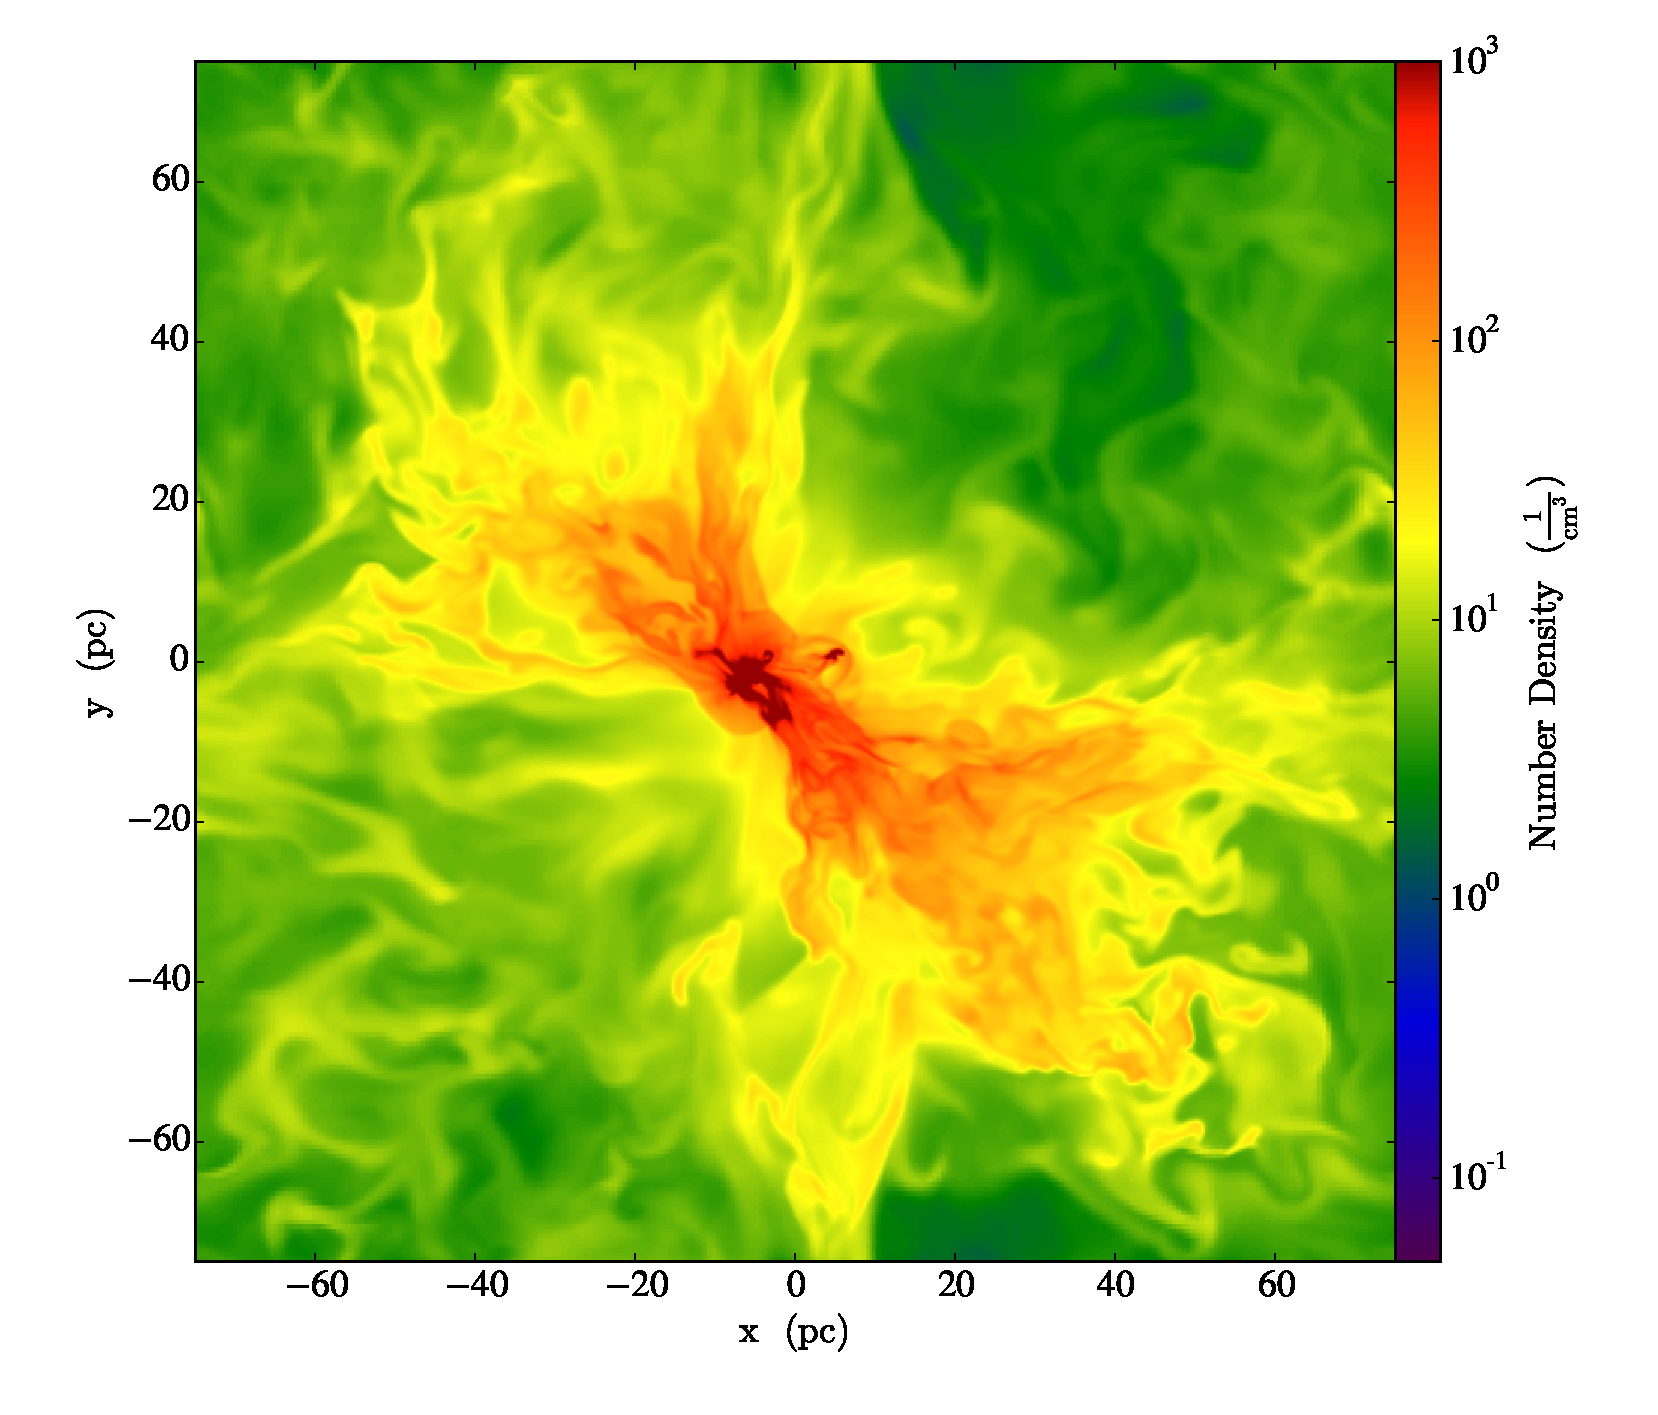
\includegraphics[width=8.5cm]{Images/density_slice}}
\end{center}
\caption{\label{fig:slice_turbulence}} Density slice at $t=19.4$ Myr for run with
cooling, turbulence, and metallicity of $Z=10^{-3}Z_\odot$. In this run cooling is
not efficient and gravity takes over forming a dense core. 
\end{figure}

 
\subsection{Heating Runs}

%% ----------------------------------------------------------------
% 
\section{Discussion}
\label{sec:discussion}
\subsection{Analytic Model}
\subsection{Implications}
\subsection{Caveats}

%% ----------------------------------------------------------------
% 
\section{Summary}

%% ----------------------------------------------------------------
% 
\section*{Acknowledgments}
\bibliography{mn-jour,gc_paper}
%
%\label{lastpage}
\end{document}
